\documentclass[11pt,letterpaper]{article}
\usepackage{fullpage}

\usepackage[english]{babel}
\usepackage[utf8]{inputenc}
\usepackage{amsmath}
\usepackage{graphicx}
\usepackage[hidelinks]{hyperref}
\usepackage{float}
\usepackage{amsfonts}
\usepackage{algorithm,algpseudocode}
\usepackage{pdfpages}
             
\graphicspath{{../results}}

\begin{document} 

\title{Experiment 2}
\maketitle

\section*{Simulation Details}

Considered $K = 3$, $T = 1001$, $N = 500$. Report statistics at $t = 1000$ \\
\textbf{The Bandit priors that were considered}:
\begin{itemize}
\item Uniform: Draw the mean rewards for the arms from [0.25, 0.75]
\item ``HeavyTail": We took the mean rewards to be randomly drawn from Beta($\alpha=0.6,\beta=0.6$). With this distribution it was likely to have arms that were at the extremes (close to 1 and close to 0) but also some of the arms with intermediate value means.
\item Needle-in-haystack
\begin{enumerate}
\item High - 2 arms with mean 0.50, 1 arm with mean 0.70 (+ 0.20)
\end{enumerate}
\end{itemize}
\textbf{Algorithms considered}:
\begin{enumerate}
\item ThompsonSampling with priors of $Beta(1, 1)$ for every arm.
\item DynamicGreedy with priors of $Beta(1, 1)$ for every arm
\item Bayesian Dynamic $\epsilon$-greedy with priors of $Beta(1, 1)$ for every arm and $\epsilon=0.05$
\end{enumerate}
\textbf{Agent Algorithms considered}:
\begin{enumerate}
\item HardMax
\item HardMaxWithRandom
\item SoftMax ($\alpha = 10$)
\end{enumerate}
\textbf{Memory Sizes}
\begin{enumerate}
\item 100
\end{enumerate}
\pagebreak
\textbf{Simulation Procedure}
\begin{algorithm}
\begin{algorithmic}[1]
\For{Each prior $p$}
\State Generate true distribution from $p$ (except for needle-in-haystack, just use $p$ itself)
\State Generate $T \times K$ realizations for the arms 
	\For{Each agent algorithm $agent alg$}
		\For{Each principal algorithm pair $principalalg1$, $principalalg2$}
			\For{$N$ simulations}
				
				\State Give the agents 5 observations from each principal
				\State Give principal 2 200 free observations (the agents also get these observations)
				\State Run simulation for T periods
			\EndFor
		\EndFor
	\EndFor
\EndFor
\end{algorithmic}
\end{algorithm}

\section*{Results}
All results are reported for memory size = 100. \\
\vspace{0.25cm}

The rows represent Principal 1 and the columns represent Principal 2. Thus, the cell (1, 2) represents principal 1 playing Thompson Sampling and principal 2 playing DynamicEpsilonGreedy. In this experiment remember that principal 2 gets 200 free observations.  \\
\vspace{0.1cm}

Within each cell, the following data are presented: \\

\begin{enumerate}
\item The first row displays the sample mean market share for principal 1 as well as a 95\% confidence band of the mean.

\item The second row displays the sample variance of the market share and in parentheses are 95 \% confidence bands for the variance.

\item The third row displays the \% of simulations that resulted in ``extreme" market shares. Extreme market shares are defined as being simulations were one of the principals (either principal 1 or 2) ended up with 90\% or more of the market.
\end{enumerate}
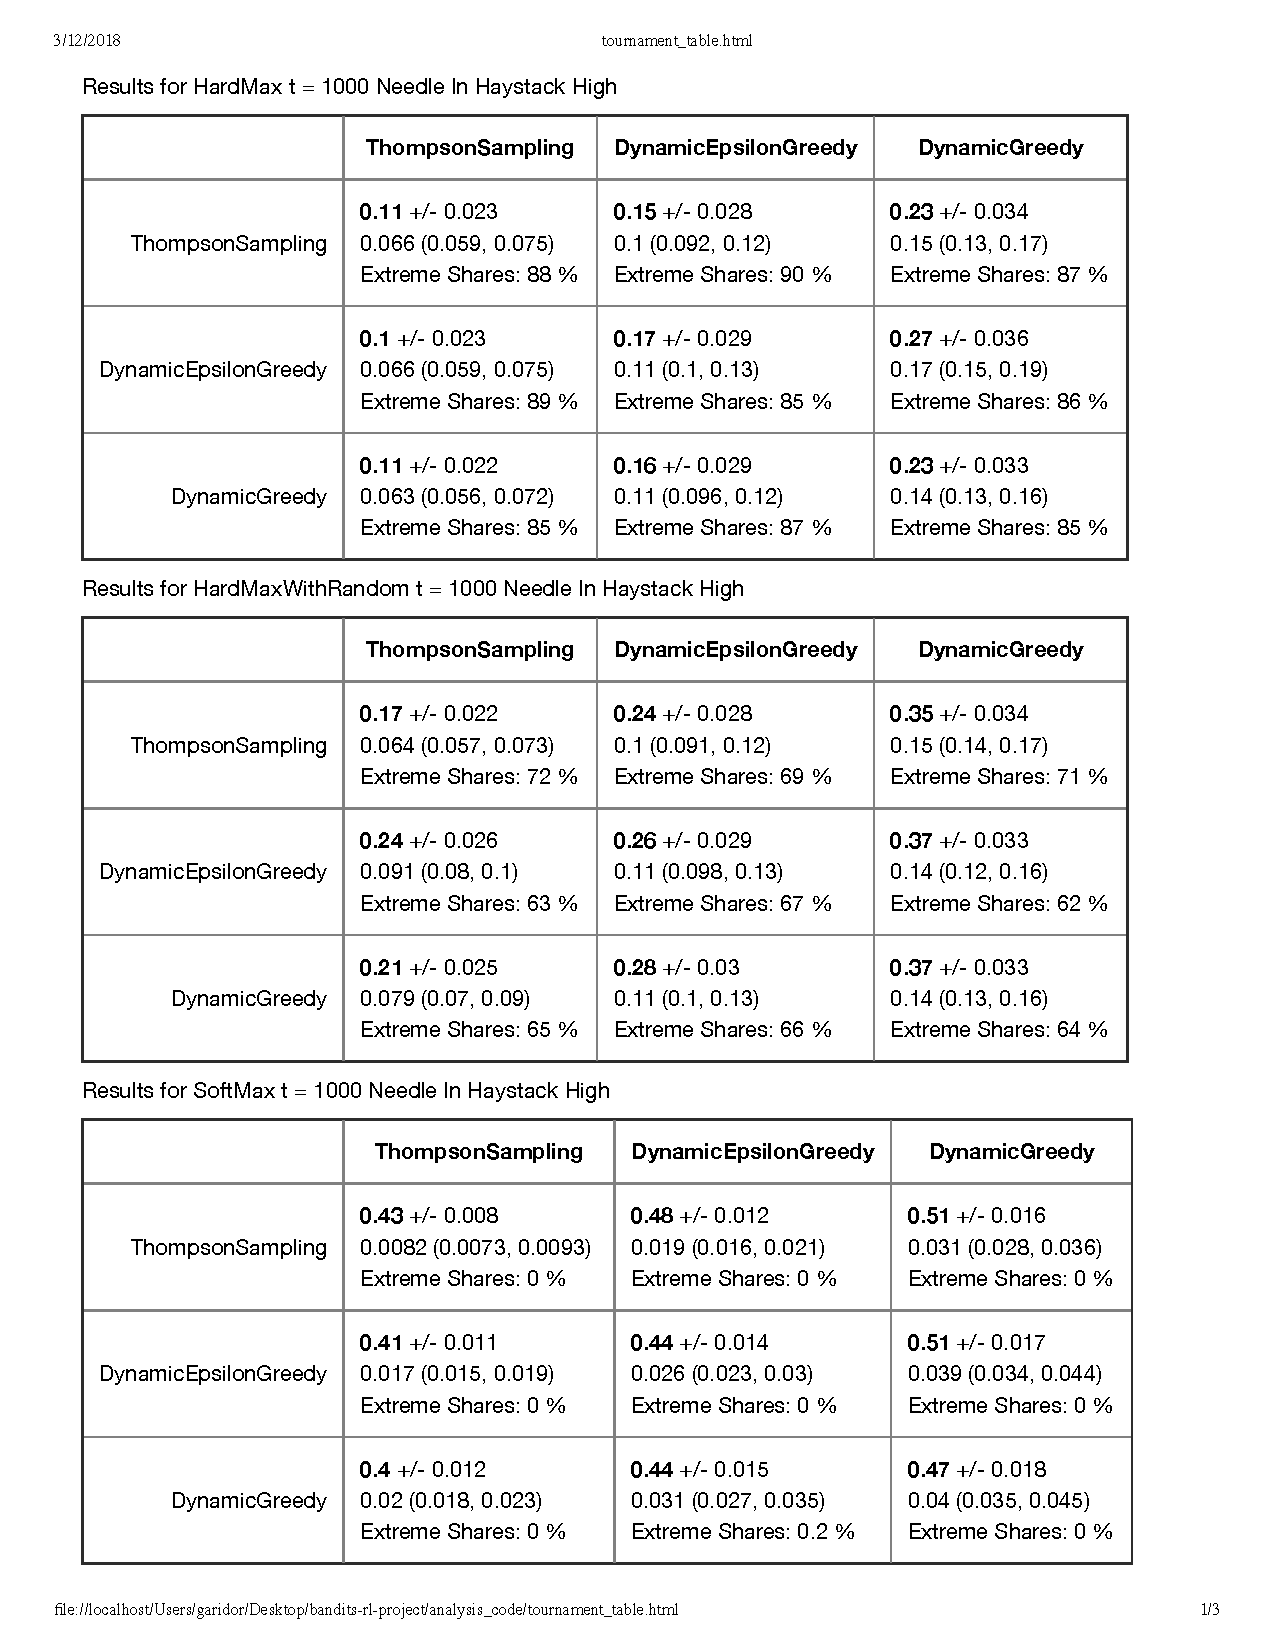
\includepdf[pages={-}]{tournament_table}

Comments: The story I seem to get from this is (roughly) that the worse the algorithm that the incumbent plays is, the better the entrant will do. However, in order for the entrant to do as well as possible, the entrant should play a worse algorithm! This seems counterintuitive, it means that the worst case for the entrant is when we're both playing ThompsonSampling and the best case for the entrant is when we're both playing DynamicGreedy.




\end{document}